\documentclass[11pt,letterpaper]{article}
\usepackage[english]{babel}
\usepackage[utf8]{inputenc}
\usepackage{fancyhdr}
\usepackage[margin=1in]{geometry}
\usepackage{enumitem}
\usepackage{amsmath}
\usepackage{graphicx}
\usepackage{setspace} 
\onehalfspacing
 
\pagestyle{fancy}
\fancyhf{}
\lhead{STAT 423 HW 4}
\rhead{Nan Tang (1662478)}
\rfoot{Page \thepage}
 

\title{STAT 423 Homework 4}
\author{Nan Tang 1662478}
\date{\today}

\begin{document}
\maketitle
\section*{1}
\subsection*{a}
\begin{verbatim}
Call:
glm(formula = purchase ~ income + age, family = binomial, data = car_dt)

Deviance Residuals: 
    Min       1Q   Median       3Q      Max  
-1.6189  -0.8949  -0.5880   0.9653   2.0846  

Coefficients:
            Estimate Std. Error z value Pr(>|z|)  
(Intercept) -4.73931    2.10195  -2.255   0.0242 *
income       0.06773    0.02806   2.414   0.0158 *
age          0.59863    0.39007   1.535   0.1249  
---
Signif. codes:  0 ‘***’ 0.001 ‘**’ 0.01 ‘*’ 0.05 ‘.’ 0.1 ‘ ’ 1
\end{verbatim}

\begin{align*}
\eta &= -4.7393 + 0.0677 \cdot income \text{( in 1000)} + 0.5986 \cdot age \\
P_{\text{buy new car}} &= \frac{1}{1 + e^{-\eta}} = \frac{1}{1 + e^{-(-4.7393 + 0.0677 \cdot income \text{( in 1000)} + 0.5986 \cdot age) }}
\end{align*}

\subsection*{b}
\noindent The estimator of $\beta_{income} = 0.0677$, the estimator of $\beta_{age} = 0.5986$. Therefore the estimated exponential for income is $1.07$, estimated exponential for age is $1.8196$. \\

\noindent Let $p$ denotes probability of buying new car, then the probability of not buying a car is $1-p$, the odds rate is $\frac{p}{1-p}$. When all other predictors remain the same, one unit of increment to income (in unit of $1000$) will increase the odds rate by $1.07$. When all other predictors remain the same, one unit of increment to age (in unit of year) will increase the odds rate by $1.8196$.

\subsection*{c}
\begin{verbatim}
> predict(fit_car1, data.frame(income=50, age=3), type='response')
0.6090245 
\end{verbatim}
\noindent The probability of this family will buy new car is $0.609$. 

\subsection*{d}
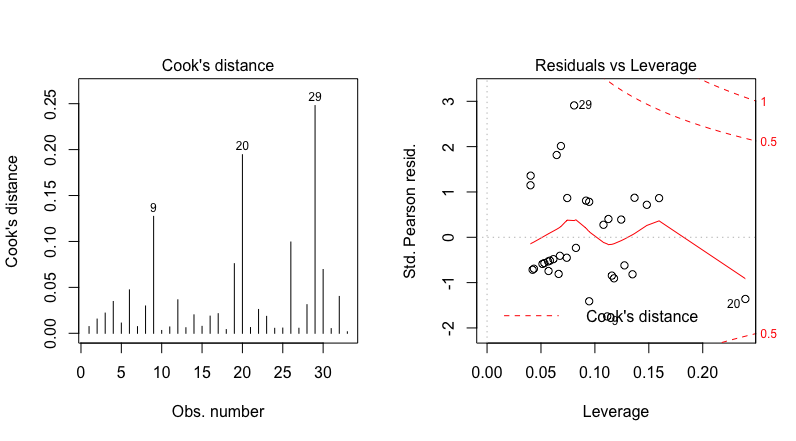
\includegraphics[scale=0.6]{1-d-1.png}

\noindent From the plots of cook's distance, we can perceive that the 20th and 29th observation have cook's distance more than 0.2. These two outliers may have more impact on regression than other points. 

\subsection*{e}
\noindent Base on z-test for coefficients of age, the z-value is 0.1249, greater than 0.05, therefore, age is not an significant predictor at the significance level of $0.05$.

\subsection*{f}
\noindent Even though the chi-square likelihood ratio test shows adding the interaction term to the model will significantly decrease deviance, the new model shows that non of the predictors are significant at level of $0.05$. Moreover, the AIC of new model is higher than original one, therefore, the interaction term is negligible in this case. 

\section*{2}
\subsection*{a}
\begin{verbatim}
resp_matrix <- data.frame(n.hyper, (n.total-n.hyper))
colnames(resp_matrix) <- c('with_hypertension', 'without_hypertension')

  with_hypertension without_hypertension
1                 5                   55
2                 2                   15
3                 1                    7
4                35                  152
5                13                   72
6                15                   36
7                 8                   15
\end{verbatim}

\subsection*{b}
\begin{verbatim}
fit_hyper1 <- glm(n.hyper/n.total~smoking+obesity+snoring, weight=n.total, family=binomial)
hyper_df <- fit_hyper1$df.residual

> pchisq(fit_hyper1$null.deviance - fit_hyper1$deviance, hyper_df, lower.tail = F)
[1] 0.006648823
\end{verbatim}

\noindent The p-value of chi-square test for residual deviance is smaller than 0.05. Implying the model has a good fitness on data. 

\subsection*{c}
\begin{verbatim}
> drop1(fit_hyper1, test='Chisq')
Single term deletions

Model:
n.hyper/n.total ~ smoking + obesity + snoring
        Df Deviance    AIC     LRT Pr(>Chi)   
<none>       1.0924 34.011                    
smoking  1   4.2010 35.120  3.1086  0.07788 . 
obesity  1   4.8781 35.797  3.7857  0.05169 . 
snoring  1  11.4062 42.325 10.3138  0.00132 **
---
Signif. codes:  0 ‘***’ 0.001 ‘**’ 0.01 ‘*’ 0.05 ‘.’ 0.1 ‘ ’ 1
\end{verbatim}

\noindent Base on ratio test, snoring is the only one significant factor under $0.05$ significance level. 

\subsection*{d}
\noindent From previous table, we can see smoking has largest p-value, indicating it is unlikely to have significant impact on response. Therefore, the first elimination will drop smoking. 

\begin{verbatim}
fit_hyper2 <- glm(n.hyper/n.total~obesity+snoring, weight=n.total, family=binomial)

> drop1(fit_hyper2, test='Chisq')

Model:
n.hyper/n.total ~ obesity + snoring
        Df Deviance    AIC    LRT Pr(>Chi)   
<none>        4.201 35.120                   
obesity  1   10.251 39.170 6.0503 0.013904 * 
snoring  1   12.303 41.222 8.1021 0.004421 **
---
Signif. codes:  0 ‘***’ 0.001 ‘**’ 0.01 ‘*’ 0.05 ‘.’ 0.1 ‘ ’ 1
\end{verbatim}

\noindent In the second elimination step, chi-square ration test indicates all of the predictors remaining significantly reduces deviance at the level of $0.05$. Therefore, we should stop here and choose the model that includes obesity and snoring as predictors. 

\subsection*{e}
\begin{verbatim}
hyper_dt <- data.frame(smoking, obesity, snoring, n.hyper, (n.total-n.hyper), (n.hyper/n.total))
colnames(hyper_dt) <- c('smoking', 'obesity', 'snoring', 'hyper', 'non_hyper', 'obs_prop')
hyper_dt <- hyper_dt %>%
  mutate(pred_prop = predict(fit_hyper2, hyper_dt[,1:3], type='response')) %>%
  mutate(pred_count = round(pred_prop * n.total)) %>%
  select(smoking, obesity, snoring, non_hyper, hyper, pred_count, obs_prop, pred_prop)
  
> hyper_dt
  smoking obesity snoring non_hyper hyper pred_count   obs_prop pred_prop
1      No      No      No        55     5          6 0.08333333 0.0938417
2     Yes      No      No        15     2          2 0.11764706 0.0938417
3      No     Yes      No         7     1          1 0.12500000 0.1834574
4     Yes     Yes      No       152    35         34 0.18716578 0.1834574
5      No      No     Yes        72    13         17 0.15294118 0.2042220
6     Yes      No     Yes        36    15         10 0.29411765 0.2042220
7      No     Yes     Yes        15     8          8 0.34782609 0.3576440
\end{verbatim}
\noindent From the comparison table, the predicted value of count is close to the real one, the model fit the data very well. 

\section*{3}
\subsection*{a}
\begin{verbatim}
data(ozone, package='gss')
set.seed(1)
ozone_dt <- ozone
ozone_dt$logupo3 <- log(ozone_dt$upo3)
ozone_dt <- select(ozone_dt, -upo3)
ozone_dt <- ozone_dt[-92,]
ff <- wrapFormula(logupo3~., data=ozone_dt, wrapString = 'poly(*, degree=3)')
ff <- update(ff, logupo3~.^3)
mm <- model.matrix(ff, data=ozone_dt)

fit_ridge <- glmnet(mm, y=scale(ozone_dt$logupo3, scale=F), alpha=0, intercept=F)
fit_lasso <- glmnet(mm, y=scale(ozone_dt$logupo3, scale=F), alpha=1, intercept=F)
fit_elnet <- glmnet(mm, y=scale(ozone_dt$logupo3, scale=F), alpha=0.5, intercept=F)

plot(fit_ridge, xvar='lambda', main='Ridge Regression')
plot(fit_lasso, xvar='lambda', main='Lasso Regression')
plot(fit_elnet, xvar='lambda',main='Elastic Net Regression')
\end{verbatim}

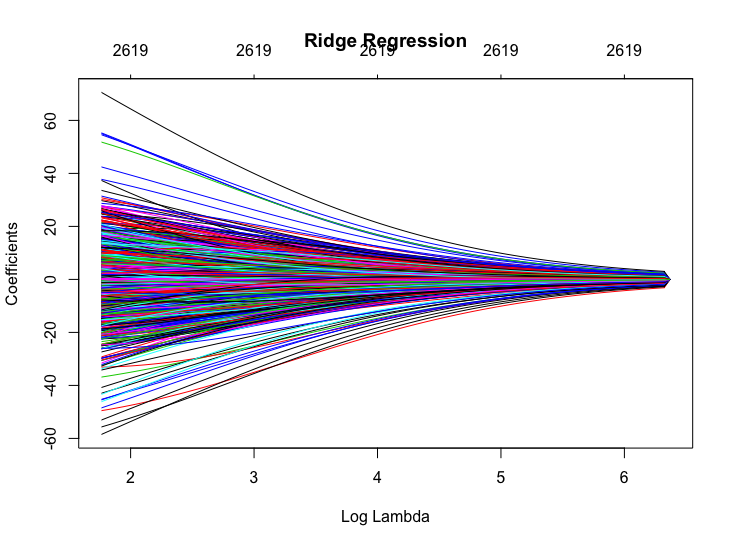
\includegraphics[scale=0.5]{3-a-1.png}

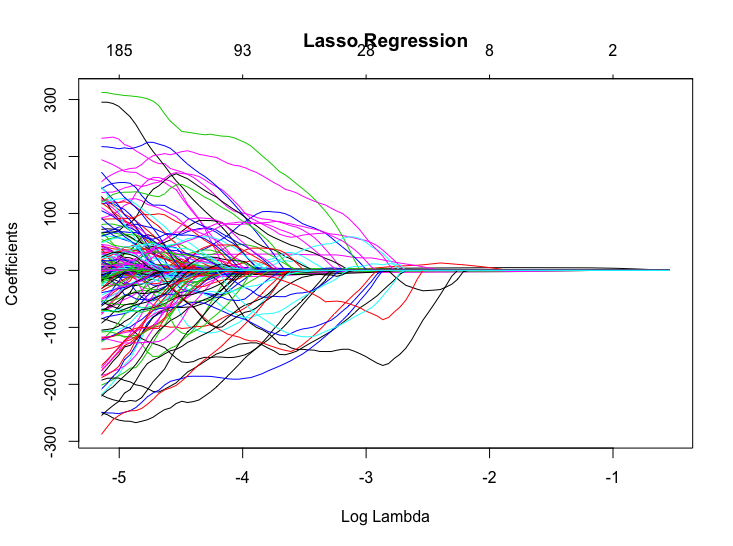
\includegraphics[scale=0.5]{3-a-2.png}

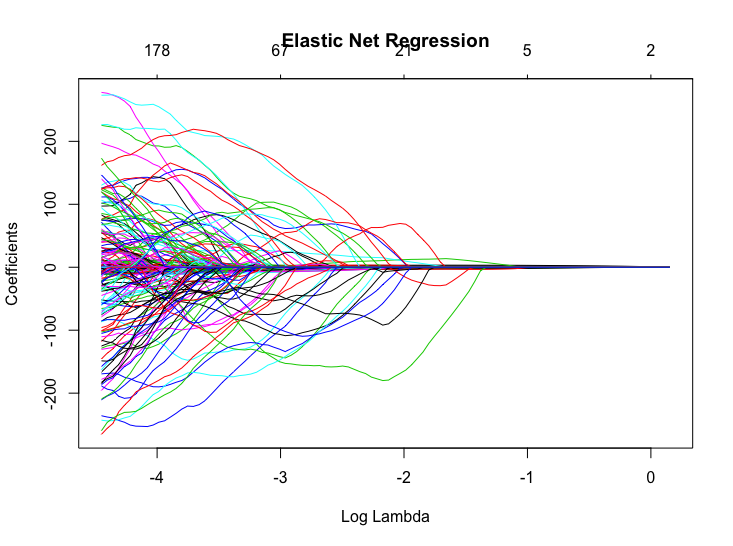
\includegraphics[scale=0.5]{3-a-3.png}

\noindent From the trace plots of Ridge Lasso and Elastic Net, we can perceive that as log lambda increases, coefficients of Ridge regression shrink monotonically to zero, while the trace for most coefficients of Lasso and Elastic Net didn't show such monotonic trend. 

\subsection*{b}
\begin{verbatim}
set.seed(1)
cv.eln <- cv.glmnet(mm, y=scale(ozone_dt$logupo3, scale=F), alpha=0.5, nfolds=10, intercept=F)
plot(cv.eln)

> cv.eln$lambda.1se
[1] 0.1088267
\end{verbatim}

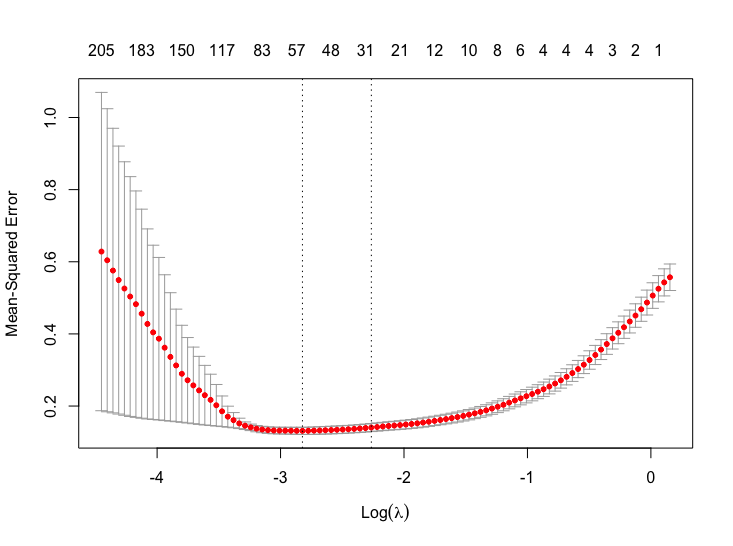
\includegraphics[scale=0.5]{3-b-1.png}

\noindent According to 1st error rule, the value of optimal lambda chosen from 10-fold cross validation is 0.1088267.

\section*{4}
\subsection*{a}
\begin{verbatim}
load('CustomerWinBack.rda')
cwb$gender <- as.factor(cwb$gender)
fitlm_cwb <- lm(data=cwb, formula=duration~.)

> summary(fitlm_cwb)
Coefficients:
             Estimate Std. Error t value Pr(>|t|)    
(Intercept) 836.15414  101.51985   8.236 6.21e-15 ***
offer       -11.91067    3.70155  -3.218  0.00144 ** 
lapse         1.09216    0.38843   2.812  0.00527 ** 
price        -8.32047    1.03278  -8.056 2.08e-14 ***
gender1     113.45371   31.73589   3.575  0.00041 ***
age           0.06461    1.08476   0.060  0.95255    
---
Signif. codes:  0 ‘***’ 0.001 ‘**’ 0.01 ‘*’ 0.05 ‘.’ 0.1 ‘ ’ 1

Residual standard error: 263.3 on 289 degrees of freedom
Multiple R-squared:   0.24,	Adjusted R-squared:  0.2269 
F-statistic: 18.25 on 5 and 289 DF,  p-value: 9.598e-16
\end{verbatim}

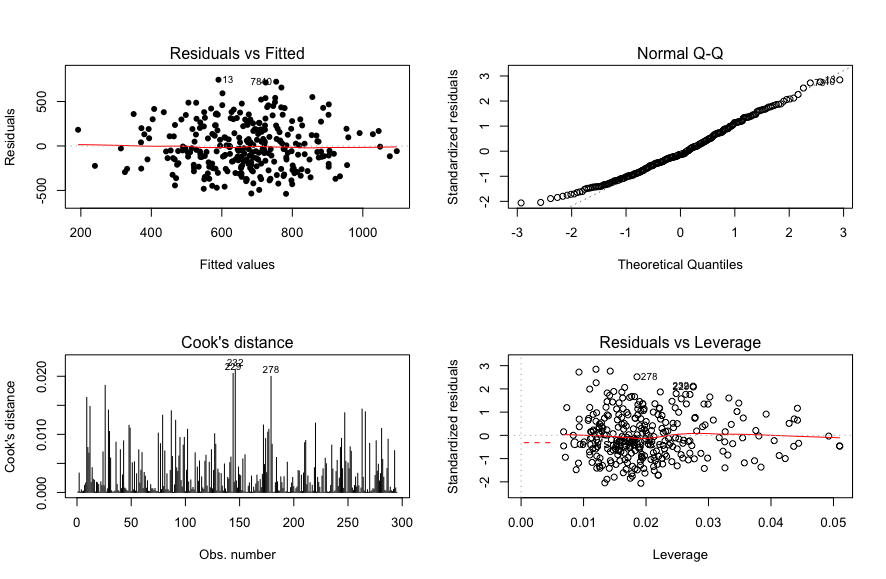
\includegraphics[scale=0.55]{4-a-1.png}

\noindent Residuals plot of OLS model shows that assumptions of constant variance and non-correlation between errors are valid. QQ plot shows the normality of error is valid. Cook's distance of each data point is less than 0.025, which is far away from 0.5, indicating there is no outlier that have great impact on regression. 

\subsection*{b}
\noindent \textbf{Backward Selection AIC}
\begin{verbatim}
step(object=fitlm_cwb, direction='backward')

Call:
lm(formula = duration ~ offer + lapse + price + gender, data = cwb)

Coefficients:
(Intercept)        offer        lapse        price      gender1  
    838.623      -11.874        1.090       -8.321      113.314  
\end{verbatim}

\noindent \textbf{Forward Selection AIC}
\begin{verbatim}
fit_empty <- lm(data=cwb, formula=duration~1)
step(object=fit_empty, direction='forward', scope=list(upper=fitlm_cwb, lowwer=fit_empty))

Call:
lm(formula = duration ~ price + gender + offer + lapse, data = cwb)

Coefficients:
(Intercept)        price      gender1        offer        lapse  
    838.623       -8.321      113.314      -11.874        1.090  
\end{verbatim}

\noindent Using AIC as criterion, both forward and backward selection will chose same model, it is $duration \sim price + gender + offer + lapse$

\subsection*{c}
\noindent \textbf{Backward Selection BIC}
\begin{verbatim}
step(object=fitlm_cwb, direction='backward', k=log(nrow(cwb)))

Call:
lm(formula = duration ~ offer + lapse + price + gender, data = cwb)

Coefficients:
(Intercept)        offer        lapse        price      gender1  
    838.623      -11.874        1.090       -8.321      113.314  
\end{verbatim}

\noindent \textbf{Forward Selection BIC}
\begin{verbatim}
step(object=fit_empty, direction='forward', k=log(nrow(cwb)),
     scope=list(upper=fitlm_cwb, lowwer=fit_empty))
     
Call:
lm(formula = duration ~ price + gender + offer + lapse, data = cwb)

Coefficients:
(Intercept)        price      gender1        offer        lapse  
    838.623       -8.321      113.314      -11.874        1.090  
\end{verbatim}

\noindent Using BIC as criterion, both forward and backward selection will chose same model, it is $duration \sim price + gender + offer + lapse$

\subsection*{d}
\begin{verbatim}
set.seed(1)
cv_ridge <- cv.glmnet(xx, yy, nfolds=5, alpha=0)
opt_lambda1 <- cv_ridge$lambda.1se
fitrg_cwb <- glmnet(xx, yy, alpha=0, lambda = opt_lambda1)
coef(fitrg_cwb)

                     s0
(Intercept) 728.9304536
offer        -3.9999010
lapse         0.4318499
price        -3.6325706
gender1      43.2353356
age          -0.1966563
\end{verbatim}

\noindent In Ridge regression, the optimized lambda is 390.6248. The model will include gender, offer, lapse, price and age. The fitted equation will be $duration = 728.93 - 3.999 \cdot offer + 0.432 \cdot lapse - 3.633 \cdot price + 42.235 \text{ if male }- 0.197 \cdot age$.


\subsection*{e}
\begin{verbatim}
set.seed(1)
cv_lasso <- cv.glmnet(xx, yy, nfolds=5, alpha=1)
opt_lambda2 <- cv_lasso$lambda.1se
fitlas_cwb <- glmnet(xx, yy, alpha=1, lambda =opt_lambda2)
coef(fitlas_cwb)

                     s0
(Intercept) 731.7021975
offer        -5.3041883
lapse         0.4706762
price        -6.6671898
gender1      61.7188198
age           .  
\end{verbatim}

\noindent In Lasso regression, the optimized lambda is 24.41. The model will include offer, lapse, price and gender . The fitted equation is $duration = 731.702 -  5.304 \cdot offer + 0.471 \cdot lapse - 6.667 \cdot price + 61.719 \text{ if male }$.

\subsection*{f}
\begin{verbatim}
pre.ols <- c() 
pre.aic <- c() 
pre.bic <- c() 
pre.rr <- c() 
pre.las <- c() 
folds <- 5
sb <- round(seq(0,nrow(cwb),length=(folds+1)))


for (i in 1:folds){
  ## define training and test datasets
  test <- (sb[((folds+1)-i)]+1):(sb[((folds+2)-i)]) 
  train <- (1:nrow(cwb))[-test]
  ## fit models
  fit.ols <- lm(duration ~ ., data=cwb[train,]) 
  fit.aic <- lm(duration ~ offer + lapse + gender + price, data=cwb[train,]) 
  fit.bic <- lm(duration ~ offer + lapse + gender + price, data=cwb[train,])
  xx <- model.matrix(duration~0+., cwb[train,])[,-4] 
  yy <- cwb$duration[train]
  fit.rr <- glmnet(xx,yy, lambda = opt_lambda1, alpha = 0) 
  
  fit.las <- glmnet(xx,yy, lambda = opt_lambda2, alpha = 1)
  ## create predictions
  pre.ols[test] <- predict(fit.ols, newdata=cwb[test,])
  pre.aic[test] <- predict(fit.aic, newdata=cwb[test,])
  pre.bic[test] <- predict(fit.bic, newdata=cwb[test,])
  pre.rr[test] <- model.matrix(duration~., cwb[test,])%*%as.numeric(coef(fit.rr)) 
  pre.las[test] <- model.matrix(duration~., cwb[test,])%*%as.numeric(coef(fit.las))
}

> mean((cwb$duration-pre.ols)^2) 
[1] 70795.21
> mean((cwb$duration-pre.aic)^2) 
[1] 70216.84
> mean((cwb$duration-pre.bic)^2) 
[1] 70216.84
> mean((cwb$duration-pre.rr)^2) 
[1] 77458.14
> mean((cwb$duration-pre.las)^2)
[1] 77727.45
\end{verbatim}

\noindent From the above cross validation, we can see the mean square error of cross validation has lowest value if choosing by AIC and BIC, indicating model chosen by stepwise fit the data best. Ridge regression has highest cross validation mean square error, implying this model fail to fit the data very well. 



\end{document}